\documentclass[11pt,a4paper]{article}

\usepackage[margin=2.3cm]{geometry}
\usepackage{amsmath,amssymb}
\usepackage{graphicx}
\usepackage{booktabs}
\usepackage{enumitem}
\usepackage[hidelinks]{hyperref}
\usepackage{caption}

\emergencystretch=1.5em
\captionsetup{font=small,labelfont=bf,width=.95\textwidth}
\setlength{\parskip}{4pt plus 1pt}
\setlength{\parindent}{0pt}

\newcommand{\code}[1]{\texttt{#1}}
\newcommand{\TopK}{\operatorname{TopK}}
\newcommand{\sign}{\operatorname{sign}}

\title{Why hard Top-$K$ with separately computed selection scores fails\\
under the code residual\\[2pt]
\large Research note}
\author{}
\date{2026-11-12.}

\begin{document}
\maketitle
\vspace{-2em}

Measurements on the \code{cairo} box (runs \code{sx\_sep\_k16\_*}, \code{sx\_sep\_k32\_*});
references from the Gumbel campaign (\code{gcr\_hard\_abs\_k16}, \code{gcr\_hard\_abs\_k32},
\code{gcr\_hard\_sep\_k16}).

\paragraph{Setup.} The model is the 8-block, 768-wide TinyStories transformer with an
activation bottleneck after every block (\code{placement: residual\_out}, $N = 1536$ code
coordinates). The bottlenecks are code-carried (\code{code\_residual: true}), have no output
norm (\code{post\_norm: false}), and train at a constant learning rate of $6\cdot10^{-4}$
after a 500-step warmup (\code{configs/gumbel\_cr/base.yaml}). Each bottleneck keeps a
\emph{support} $S_l$ of exactly $K$ coordinates, given by a hard binary mask $m_l$. Two ways
of choosing the support are compared:
\begin{itemize}[leftmargin=1.5em,itemsep=2pt]
  \item \textbf{abs-TopK} (\code{selection\_mode: abs\_topk}): $S_l$ holds the $K$
    coordinates of largest magnitude $|a_i|$ of the code $a$ itself.
  \item \textbf{Separate scores} (\code{selection\_mode: learned\_score\_topk}): an
    independent linear scorer $s = W_s h + b_s$ reads the residual-stream state $h$, and
    $S_l$ holds the $K$ largest $s_i$. The code values $v = a$ are kept unscaled on $S_l$.
    The mask passes no gradient to $s$, so the scorer is trained by the \emph{support
    gradient}
    $\partial L/\partial s_i = \mathbf 1[i \in S]\,\sign(v_i)\,\partial L/\partial y_i$,
    with $y = v \odot m$ the bottleneck output.
\end{itemize}

The separate-score runs failed for two reasons, and each has a fix. With both fixes the runs
train, but they still trail abs-TopK.

\begin{figure}[h]
  \centering
  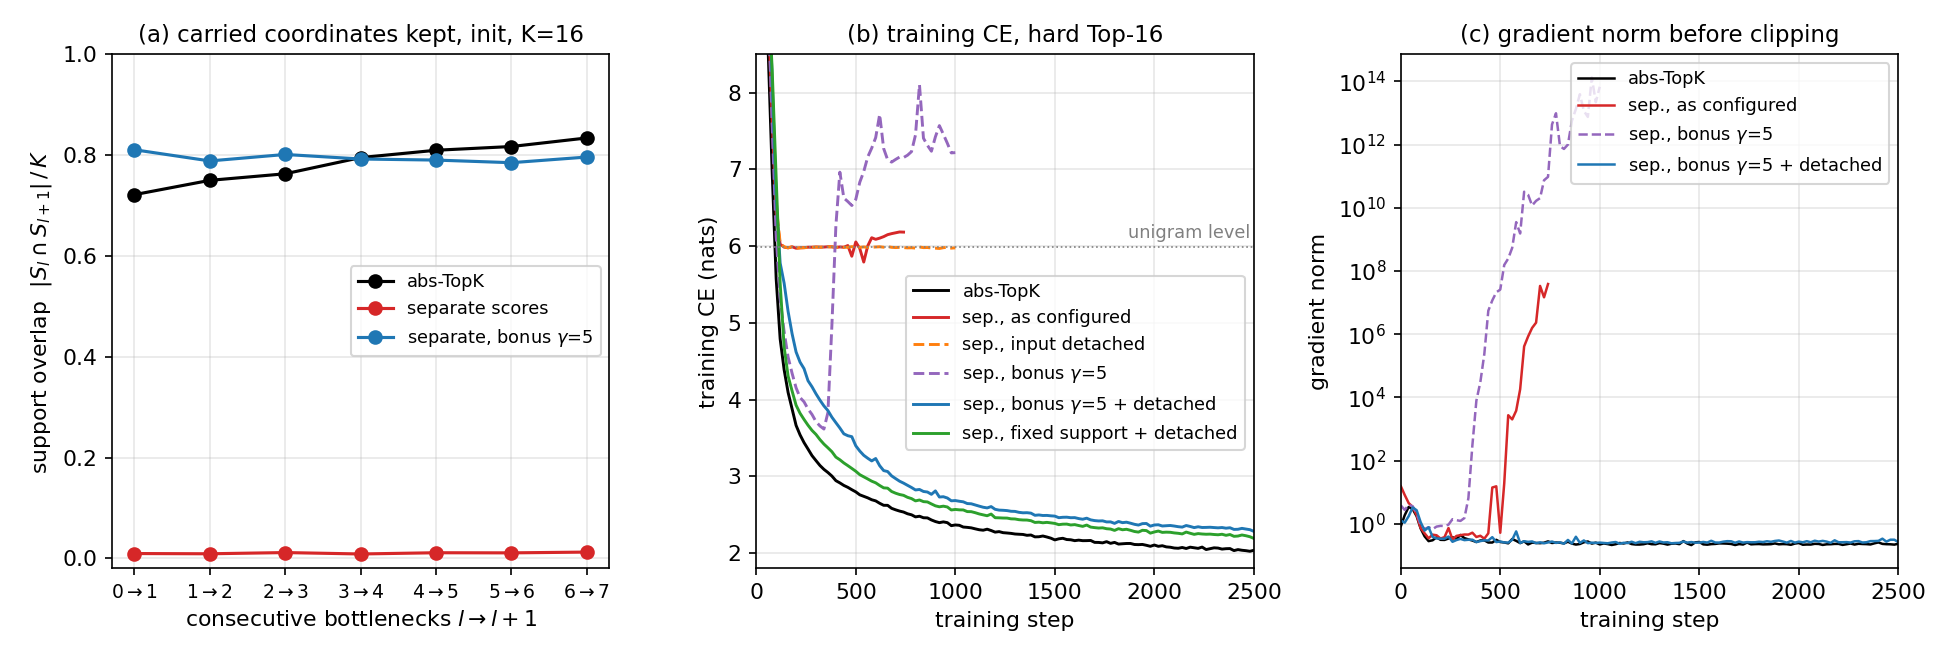
\includegraphics[width=\textwidth]{figures/separate-score/separate_score_failure.png}
  \caption{(a) Share of the carried coordinates that the next bottleneck keeps, at
  initialization, $K = 16$. (b) Training CE of hard Top-16 in six configurations; the
  dotted line is the unigram level (5.99 nats). (c) Gradient norm before clipping, log
  scale. The as-configured run was stopped at step 740.}
  \label{fig:main}
\end{figure}

\section{The independent scores cut the code skip, so training stalls at the unigram level}

Under the code residual, a block's input reaches later blocks only through the carried code
$c_l$, on the coordinates the next support keeps:
\begin{equation}
  x_{l+1} = D\,c_{l+1}, \qquad c_{l+1} = (c_l + E\,\Delta_l)\odot m_{l+1},
\end{equation}
where $x_{l+1}$ is the stream block $l+1$ reads, $\Delta_l$ the output of block $l$'s
attention and MLP branches, and $E$, $D$ the bottleneck's encoder and decoder. abs-TopK
selects the large carried coordinates again, because they dominate $c_l + E\Delta_l$. A
randomly initialized scorer selects independently of $c_l$, so consecutive supports share
about $K/N$ of their coordinates: 0.010 at $K = 16$, against 0.78 for abs-TopK
(Figure~\ref{fig:main}a). The skip path is gone at initialization.

\textbf{Fix:} a bonus on the scores of the coordinates the carried code occupies,
\begin{equation}
  s_l \leftarrow s_l + \gamma\,\mathbf 1[c_l \neq 0] \qquad (l \ge 1)
\end{equation}
(\code{learned\_score\_carry\_bonus:}~$\gamma$). $\gamma = 5$ restores an overlap of 0.80. A
very large $\gamma$ fixes the support after block 0.

\section{The scorer's support gradient flowing into the trunk makes training diverge}

$s$ affects the loss only through ranking. So the term
$W_s^{\top}\big(\sign(v)\odot\partial L/\partial y\big)$ that the support gradient sends into
$h$ is not a gradient of the loss, and it grows with $\|W_s\|$, which it also inflates. The
score gap and the gradient norm grow without bound, to about $10^{14}$
(Figure~\ref{fig:main}c), and training diverges (Figure~\ref{fig:main}b, carry bonus alone).

\textbf{Fix:} detach $h$ in the scorer (\code{learned\_score\_input\_grad: false}). The
scorer still learns from the support gradient; the trunk gets none of it.

\section{Results}

Validation CE of separate-score hard Top-16 (abs-TopK hard Top-16: 2.39 at step 1000):

\begin{center}
\begin{tabular}{ll}
\toprule
variant & val CE at 1000 \\
\midrule
as configured & 5.99 (stall), then diverges; stopped at step 740 \\
scorer input detached only & 5.99 \\
carry bonus only ($\gamma = 5$) & 4.13 at step 200, then diverges \\
carry bonus, scorer frozen & 3.78 \\
carry bonus + detached input & 2.70 \\
support fixed after block 0 + detached input & 2.59 \\
\bottomrule
\end{tabular}
\end{center}

At step 2500 the fixed runs still lag abs-TopK:

\begin{center}
\begin{tabular}{lcc}
\toprule
run & val CE at 2500 & abs-TopK at 2500 \\
\midrule
Top-16, $\gamma = 5$ + detached input & 2.338 & 2.064 \\
Top-16, support fixed after block 0 + detached input & 2.249 & 2.064 \\
Top-32, $\gamma = 5$ + detached input & 2.124 & 1.959 \\
\bottomrule
\end{tabular}
\end{center}

All runs are single runs at seed 1337. What causes the remaining 0.17--0.27 nats has not
been investigated.

\paragraph{Code and data.}
{\raggedright
\begin{itemize}[leftmargin=1.5em,itemsep=1pt]
  \item config fields \code{learned\_score\_carry\_bonus} (default 0) and
    \code{learned\_score\_input\_grad} (default true);
  \item the overlap measurement: \code{analysis/code\_carry\_overlap.py};
  \item the figure: \code{scripts/plot\_separate\_score\_failure.py}, data in
    \code{docs/figures/separate-score/data/};
  \item runs on Drive: \code{runs\_cairo/sx\_*}, \code{runs\_bern/gcr\_hard\_sep\_k16},
    \code{runs\_ankara/gcr\_hard\_abs\_k16}.
\end{itemize}
}

\end{document}
